We begin by considering the phenomenon of increasing efficiency in repeated reference games: speakers use detailed descriptions at the outset but converge to an increasingly compressed shorthand while remaining understandable to their partner.
While this phenomenon has been extensively documented, to the point of serving as a proxy for measuring common ground, it has continued to pose a challenge for models of communication.

  \begin{figure*}
\centering
    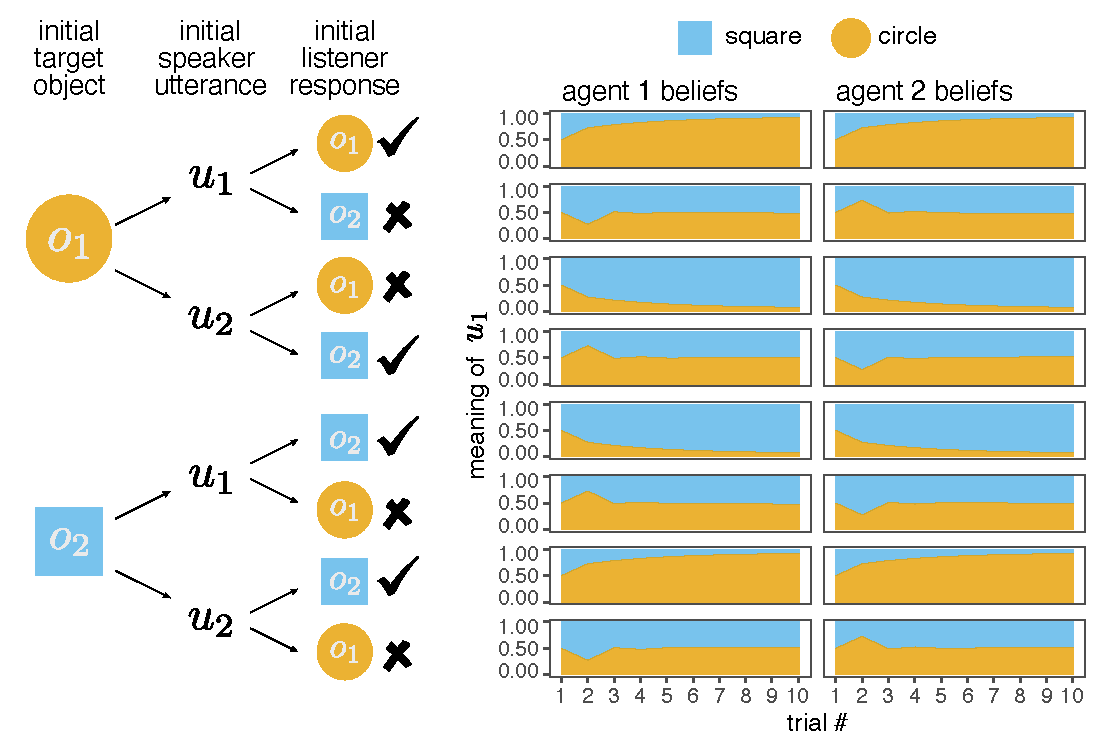
\includegraphics[scale=.8]{sec1-arbitrariness}
    \vspace{1em}
    \caption{\emph{Path-dependence of conventions.} The average trajectory of each agent's beliefs about the meaning of $u_1$, $\phi(u_1)$, are shown following all eight possible outcomes of the first trial in Simulation 1.1. For each of the two possible targets, the speaker could choose to produce either of the two utterances, and the listener could respond by choosing either of the two objects. In the cases where the listener chose correctly (marked with a checkmark), agents subsequently conditioned on the same data and rapidly converged on a system of meaning consistent with this feedback. For example, in the first row, when $u_1$ was successfully used to refer to the circle, both agents subsequently believe that $u_1$ means \emph{circle} in their partner's lexicon. In the cases where the listener fails to choose the target, the agents subsequently condition on different data, and they converge on a convention that is determined by later choices (lines represent the trajectories of individual agents.)}
  \label{fig:path-dependence}
\end{figure*}

For example, one possibility is that speakers coordinate on meaning through priming mechanisms at lower levels of representation, as proposed by influential  \emph{interactive alignment} accounts \cite{pickering2004toward, pickering2006alignment, garrod2009joint}.
While low-level priming may be at play in repeated reference tasks, especially when listeners engage in extensive dialogue or alternate roles, it is not clear why priming would cause descriptions to get shorter as opposed to aligning on the same initial description.
Furthermore, priming alone cannot explain why speakers still converge to more efficient labels even when the listener is prevented from saying anything at all and only minimal feedback is provided showing that the listener is responding correctly \cite{KraussWeinheimer66_Tangrams}; conversely, speakers continue using longer descriptions when they receive non-verbal feedback that the listener is repeatedly making errors \cite<see also>{hawkins2020characterizing}.
In these cases, there are no linguistic features available for priming or alignment mechanisms.
Explaining when and why speakers believe that shorter descriptions will suffice requires a mechanism for coordination on meaning even given sparse, non-verbal feedback.


Another possibility is that speakers coordinate on meaning using some some lexical update rule that makes utterances more likely to be produced after communicative successes and less likely after communicative failures, such as a variant on the Roth-Erev reinforcement learning rule \cite{erev1998predicting} adopted by a variety of agent-based models \cite{steels_self-organizing_1995,barr_establishing_2004,young_evolution_2015}.
While reinforcement is a powerful mechanism for allowing groups to reach consensus, it is not clear why a newly initialized speaker would prefer to produce longer utterances over shorter utterances, or, if this bias was built-in, how simply reinforcing initially long descriptions could lead utterances to get shorter. 
In the rare cases that some form of reduction has been investigated in this family of models (e.g. as in the phenomenon of phonological erosion), the process has been hard-coded as an $\epsilon$ probability of speakers dropping a random token at each point in time \cite{beuls2013agent,steels2016agent}.


Such random dropping, however, is an unsatisfying explanations for several reasons.
First, it formalizes a reductive explanation of efficiency in terms of speaker-internal noise (or laziness). This idea dates back to the early literature on repeated reference games and
control experiments by \citeA{HupetChantraine92_CollaborationOrRepitition} were designed to test this possibility \cite<see also>{GarrodFayLeeOberlanderMacLeod07_GraphicalSymbolSystems}. 
Participants were asked to repeatedly refer to the same targets for a \emph{hypothetical} partner to see later, such that any effects of familiarity or repetition on the part of the speaker were held constant with the interactive task. 
No evidence of reduction was found, and in some cases utterances actually grew longer.
This accords with observations in multi-partner settings by \citeA{wilkes-gibbs_coordinating_1992}, which we explore further in \textbf{P2}: it is difficult to explain why a speaker who only shortened their descriptions due to an $\epsilon$-noise process would suddenly switch back to a longer utterance when their partner is exchanged.
Whatever drives efficiency cannot be explained through speaker laziness, it must be a result of the \emph{interaction} between partners.


In this section, we argue that our Bayesian account provides a rational explanation for increasing efficiency in terms of the inferences made by speakers across repeated interaction.
Given that this phenomenon arises in purely dyadic settings, it also provides an opportunity to explore more basic properties of the first two capacities formalized in our model (representing \emph{uncertainty} and \emph{partner-specific learning}) before introducing hierarchical generalization in the next section. 
In brief, we show that increasing efficiency is a natural consequence of the speaker's tradeoff between informativity and parsimony (Eq.~\ref{eq:marginalized}), given their inferences about the listener's language model. 
For novel, ambiguous objects like tangrams, where speakers do not expect strong referential conventions to be shared, longer initial descriptions are motivated by high initial uncertainty in the speaker's lexical prior $P(\phi_k | \Theta)$. 
Proposing multiple descriptors is a rational hedge against the possibility that any particular meaning is not shared by the listener.
\ndg{our model doesn't exactly do this "rational hedge" thing -- see comments below -- should we stick with that description?}
As the interaction goes on, the speaker obtains feedback $D_k$ from the listener responses and updates their posterior beliefs $P(\phi_k | D_k)$ accordingly. 
As uncertainty gradually decreases, they are able to achieve the same expected informativity with shorter, more efficient messages. 


\subsection{Simulation 1.1: Pure coordination}


We build up to our explanation of increasing efficiency by first exploring a traditional signaling game scenario with only one-word utterances.
This simulation tests the most fundamental competency for any model of \emph{ad hoc} coordination: agents are able to coordinate on a communication system in the absence of shared priors. 
We consider the simplest possible reference game with two objects, $\mathcal{O} = \{\orangecircle, \bluesquare\}$, where the speaker must choose between two one-word utterances $\mathcal{U} = \{u_1, u_2\}$ with equal production cost. 

We walk explicitly through the first step of the simulation to illustrate the model's dynamics (see Fig.~\ref{fig:path-dependence}).
Suppose the target object presented to the speaker agent on the initial trial is $\orangecircle$.
Both utterances are equally likely to apply to either object under the uniform lexical prior, hence each utterance is expected to be equally (un)informative. 
The speaker's utility therefore reduces to sampling an utterance at random $u~\sim~S(u\,|\, \orangecircle)$.
Suppose $u_1$ is sampled.
The listener then hears this utterance and selects an object according to their own expected utility under their uniform lexical prior, which also reduces to sampling an object at random $o \sim L(o | u_1)$.
Suppose they choose, $ \orangecircle$, a correct response.
Both agents may use the resulting tuple $D = \{ \orangecircle^*, u_1,  \orangecircle\}$, depicted in the top row in Fig.~\ref{fig:path-dependence} to update their beliefs about the lexicon their partner is using.
\begin{align}
P_S(\phi | D) & \propto L_0( \orangecircle\, |\, u_1, \phi)P(\phi)\nonumber \\
P_L(\phi | D) & \propto S_1(u_1 \,|\, \orangecircle^*, \phi)P(\phi)\nonumber
\end{align}
They then proceed to the next trial, where they use this updated posterior distribution to produce or interpret language instead of their prior.
To examine how the dynamics of this updating process unfold over further rounds, we simulated 1000 such trajectories.
The trial sequence was structured as a repeated reference game, containing 30 trials structured into 15 repetition blocks.
The two objects appeared in a random order within each block, and agents swapped roles at the beginning of each block.
We show representative behavior at soft-max optimality parameter values $\alpha_L = \alpha_S = 8$ and memory discounting parameter $\beta = 0.8$, but find similar behavior in a wide regime of parameter values (see Appendix Fig.~\ref{fig:arbitrariness_grid}).


\begin{figure}[t]
\centering
    \includegraphics[scale=.8]{sec1-convergence.pdf}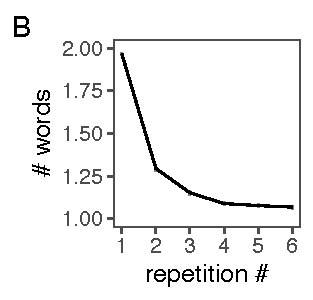
\includegraphics[scale=.8]{sec1-efficiency}
  \caption{\emph{Pairs of agents learn to successfully coordinate on efficient ad hoc conventions over repeated interactions.} (A) agents converge on accurate communication systems in Simulation 1.1, where only single-word utterances are available, and (B) converge on shorter, more efficient conventions in Simulation 1.2, where multi-word utterances were available. Error bars are bootstrapped 95\% CIs across 1000 trajectories, computed within each repetition block of two trials.}
  \label{fig:sec1model}
\end{figure}


We highlight several key results from this simulation.
First, and most fundamentally, the communicative success of the dyad rises over the course of interaction: the listener is able to more accurately select the intended target object (see Fig.~\ref{fig:sec1model}A). 
Second, the initial symmetry between meanings in the prior is broken by initial choices, leading to \emph{arbitrary} but \emph{stable} mappings in future rounds.
Because agents were initialized with the same priors in every trajectory, trajectories only diverged when different actions happen to be sampled.
This can be seen by examining the path-dependence of subsequent beliefs based on the outcome of the initial trial in Fig.~\ref{fig:path-dependence}.
Third, we observe the influence of mutual exclusivity via Gricean pragmatic reasoning: agents also make inferences about objects and utterances that were \emph{not} chosen. 
For example, observing $D = \{(\orangecircle^*, u_2, \orangecircle)\}$ provides evidence that $u_1$ likely does not mean $\orangecircle$ (e.g.~the third row of Fig.~\ref{fig:path-dependence}, where hearing $u_2$ refer to $\orangecircle$ immediately led to the inference that $u_1$ likely refers to $\bluesquare$).

\subsection{Simulation 1.2: Increasing efficiency}

Next, we show how our model explains speakers' gains in efficiency over multiple interactions. 
For efficiency to change at all, speakers must be able to produce utterances that vary in length. 
For this simulation, we therefore extend the model to allow for multi-word utterances by allowing speakers to combine together multiple primitive utterances.
Human speakers essentially form long description by proposing a collection of simpler descriptions (e.g. ``kind of an X or maybe a Y with Z on top''). 
This behavior suggests that multi-word utterances $u_iu_j$ ought to be interpreted according to a `max' operation, allowing the literal listener to use any component part that fits the referent under the given lexicon\footnote{We focus on the `max' operation as one of the simplest and most natural ways of constructing longer, non-atomic utterances from primitives. See also \citeA{SteinertThrelkeld16_CompositionalSignaling} who consider the operation of negation. We discuss the possibility of a conjunctive operation in Appendix B, which is capable of producing the desired increases in efficiency but requires additional assumptions about strategically ``failing to refer'' that we find implausible.}:
$$\mathcal{L}_\phi(u_iu_j, o) = \max\{\mathcal{L}_\phi(u_i, o) , \mathcal{L}_\phi(u_j, o)\}$$
\ndg{pre-discussion comment: earlier we defined $\mathcal{L}$ to be Boolean valued, so it's not clear what $\max$ means. i believe we mean "logical OR"? maybe just call it OR? Also... people will be confused by this because it is not how binomial constructions actually work in language. I think we are driven to it because we don't have any "neutral" options where i can just say i'm not sure what u1 means so it doesn't contribute to the full utterance meaning. this could come from a soft semantics (ie then we have 0.5 available and product should be ok), or from composing at the level of distributions...}
\ndg{updated thoughts post-discussion: i *really* don't like the logical-or semantics (aka MAX rule, but we are working with boolean denotations, so it's just OR) because it leads to some very unintended consequences if we make the world of the simulation just a bit more complex. eg if there were color and shape properties, we really want [[red square]] = [[red]] AND [[square]] (and not [[red]] OR [[square]]). so we would need some unusual semantic rules anyhow -- "OR if the predicates refer to the same feature, AND if different". at which point i think it's nicer to just be explicit that we want this kind of "modal conjunction" whose meaning is AND except if it's false for all possible referents, when it's true (or equivalently neutral if we had a third value).
btw i should flag that i'm happy enough with this "modal and" approach for the paper, but i actually think it derives the initial preference for two words for the wrong reason. essentially, in this approach (and the OR one) the S1 chooses "u1u2" because this leads the L0 to not update her beliefs when u1 contradicts u2, and this is preferable to risking L0 having the wrong belief (because log is asymmetric, so log(0) is a really bad utility). i think we all share the intuition that why the speaker should actually produce two words is to hedge her bets on one word not being understood as she expects -- "u1u2" should be more likely to convey the correct meaning, not just be a noop. we could get the hedging (aka rational redundancy) effect if either we had soft semantics with product or max composition, or if there was some chance that each word is true of both objects. (robert, did we talk through that latter option -- putting some probability mass on the lexicon [[0,1],[1,1]] etc? there may be some reasons it doesn't work?) but i think robert convinced me that following down this route is too complicated in terms of inference (distributions on continuous semantics) and model description (non-truth functional semantics or uncertainty in more places), and not really needed for the purposes of this paper.
}

Now, we consider a scenario with the same two objects as in Simulation 1.1, but give the speaker four primitive utterances $\{u_1, u_2, u_3, u_4\}$ instead of only two, and allow two-word utterances, $u_1u_2$ etc. 
We established in the previous section that successful \emph{ad hoc} conventions can emerge even in a state of pure uncertainty, but human participants in repeated reference games typically bring some prior expectations about language into the interaction.
For example, a participant who hears `ice skater' on the first round of the task in \citeA{ClarkWilkesGibbs86_ReferringCollaborative} may be more likely to select some objects more than others while still having substantial uncertainty about the intended target (e.g. over three of the twelve tangram that have some resemblance to an ice skater).
This observation is key to understanding why speakers may initially use longer utterances in repeated reference games with ambiguous stimuli. 
Under a completely uniform prior, where all words are expected to be equally meaningless to one's partner, longer utterances have no additional value. 

\ndg{could you confirm that last sentence is true of our current model? because the model is using "u1u2" to be a noop, in order to avoid L0 having a false belief, it may actually choose "u1u2" more even if the meanings are uniform??}
Under a completely concentrated prior, where there already exists a strong convention for a short label, that label would suffice and a longer utterance is redundant.
We thus initialize both agents with very weak biases (represented in compressed matrix form in Fig.~\ref{fig:sec1efficiency}):
\begin{align}
\phi(u_1), \phi(u_2) \sim \textrm{Categorical}(0.5 + \delta) \nonumber\\
\phi(u_3), \phi(u_4) \sim \textrm{Categorical}(0.5 - \delta) \nonumber
\end{align}

\begin{figure}
\centering
    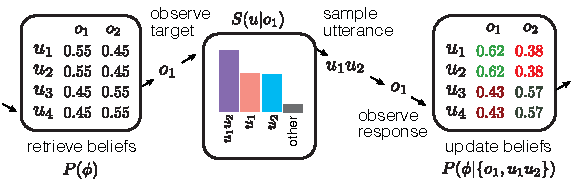
\includegraphics[scale=.87]{sec1-reduction_example}
    \vspace{1em}
  \caption{\emph{Schematic of speaker for first trial of Simulation 1.2.} The speaker begins with uncertainty about the meanings in the listener's lexicon (e.g. assigning 55\% probability to the possibility that utterance $u_1$ means object $o_1$.) A target $o_1$ is presented, and the speaker samples an utterance from the distribution $S(u|o_1)$. Finally, they observe the listener's response and update their beliefs. Due to the compositional semantics of the utterance $u_1u_2$, the speaker becomes increasingly confident that both component primitives, $u_1$ and $u_2$, apply to object $o_1$ in their partner's lexicon.}
  \label{fig:sec1efficiency}
\end{figure}

%\begin{figure}[b]
%\centering
%  \caption{\emph{Agent converge on more efficient utterances over repeated interactions.} Error bars are bootstrapped 95\% CIs across 1000 simulated trajectories.}
%  \label{fig:sec1efficiency}
%\end{figure}


\begin{figure*}[t]
\centering
    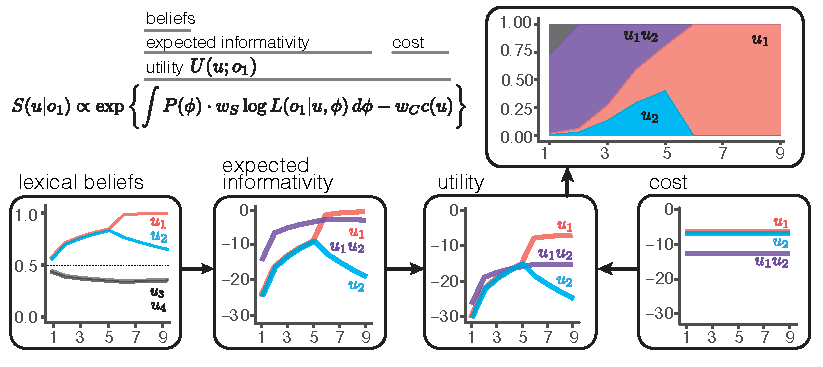
\includegraphics[scale=1.2]{sec1-reduction_schematic}
    \vspace{1em}
  \caption{\emph{Internal state of speaker in example trajectory from Simulation 1.2.} Each term of the speaker's utility (Eq. \ref{eq:marginalized}) is shown throughout an interaction. When the speaker is initially uncertain about meanings (far left), the longer utterance $u_1u_2$ has higher expected informativity (center-left) and therefore higher utility (center-right) than the shorter utterances $u_1$ and $u_2$, despite its higher cost (far-right). As the speaker observes several successful interactions, they update their beliefs and become more confident about the meanings of the component lexical items $u_1$ and $u_2$. As a result, more efficient single-word utterances gradually gain in utility as cost begins to dominate the utility. On trial 5, $u_1$ is sampled, breaking the symmetry between utterances.}
  \label{fig:sec1internals}
\end{figure*}

As in Simulation 1.1, we simulated 1000 distinct trajectories of dyadic interaction between agents.
Utterance cost was defined to be the number of `words' in an utterance, so $c(u_1) =1$ and $c(u_1u_2)=2$.
Our speaker agent initially prefers longer utterance (mean length $\approx 1.5$ on first block) but rapidly converges to shorter utterances after several repetitions (mean length $\approx 1$ on final block), qualitatively matching the curves measured in the empirical literature (Fig.~\ref{fig:sec1model}B).

To illustrate in detail how our model derives this phenomenon, we walk step-by-step through a single trial (Fig. \ref{fig:sec1efficiency}).
Consider a speaker who wants to refer to object $o_1$. 
They expect their partner to be slightly more likely to interpret their language using a lexicon in which $u_{1}$ and $u_{2}$ apply to this object, due to their weak initial biases. 
However, there is still a reasonable chance ($p=0.45$) that either $u_1$ or $u_2$ alone will be interpreted to mean $o_2$ by their partner, which would lead to an incorrect response. 
Thus, it is more informative to produce the longer utterance $u_{1}u_{2}$ to hedge against this possibility, despite its higher production cost. 

\ndg{ok, we need to be careful / add more explanation here. the real reason the speaker chooses the two word utterance isn't exactly to make sure one of the words conveys the correct meaning, it's to make sure that the listener doesn't get a false belief --- this is bad because of the shape of log -- and the two word utterance yields no belief update when the words contradict each other.}
To see why this is the case, consider the expected informativity of the utterance under different possible listener lexicons.
The possibility with highest probability is that both $u_1$ and $u_2$ will mean $o_1$ in the listener's lexicon ($p = 0.55^2 \approx 0.3$), in which case the listener will correctly identify the target with high probability.
The possibility that both $u_1$ and $u_2$ will mean $o_2$ in the listener's lexicon is only $p=0.45^2 \approx 0.2$, leading the listener to erroneously select $o_2$ with high probability. 
In the mixed cases, where just one of $u_1$ or $u_2$ means $o_2$ in the listener's lexicon ($p = 2 \cdot 0.45 * 0.55 \approx 0.5$), the listener will choose between the objects at chance, which yields an intermediate informativity.
When expected informativity is calculated across these outcomes, it is more valuable to produce the longer disjunction than the shorter component utterances.
Finally, upon observing the listener's response to the disjunction (say, $o_1$), the speaker becomes more confident that the component utterances $u_1$ and $u_2$ mean $o_1$ in their updated posterior over the listener's lexicon.
This credit assignment to individual lexical items is a consequence of the compositional meaning of longer utterances in our simple grammar.
\ndg{would be good to unpack that last point with another sentence or two. eg "the speaker knows a listener for whom either $u_1$ or $u_2$ means $o_1$ would have been likely to make the observed choice, and so the probability of those mappings increases."}
As shown in Fig.~\ref{fig:sec1model}B, our speaker agent initially prefers longer utterance (mean length $\approx 1.5$ on first block) but rapidly converges to shorter utterances after several repetitions (mean length $\approx 1$ on final block), qualitatively matching the curves measured in the empirical literature (e.g. Fig.~\ref{fig:clark92}).

Fig.~\ref{fig:sec1internals} shows the trajectories of internal components of the speaker utility as the interaction continues.
We assume for illustrative purposes that $o_1$ continues to be the target on each trial and the same agent continues to be the speaker.
As the posterior probability that individual primitive utterances $u_1$ and $u_2$ independently mean $o_1$ increases (far left), the marginal gap in informativity between the disjunction and the shorter components gradually decreases (center left).
As a consequence, production cost increasingly dominates the utility (center-right). 
After several trials of observing a successful listener response given the disjunction, the utility of the shorter utterances reaches parity with the disjunction (yielding a situation now similar to Simulation 1.1).
Once the speaker samples a shorter utterance (e.g. $u_1$), the symmetry collapses and that utterance remains most probable in future rounds, allowing for a stable and efficient \emph{ad hoc} convention.
Thus, increasing efficiency is derived as a rational consequence of uncertainty and partner-specific inference about the listener's lexicon.
For these simulations, we used $\alpha_S = \alpha_L = 8, w_c = 0.24, \beta=0.8$ but the qualitative reduction effect is found over a range of different parameters (see Appendix Fig. \ref{fig:conjunction_grid}). 
%\paragraph{Model comparison}
%
%Here we compare this model to several simpler baselines to establish which components of the model are necessary and sufficient for the desired behavior.
%
%\rdh{e.g., no pragmatics, pragmatics only in learning rule or only in decision rule instead of both, simpler pragmatics (reasoning about $L_0$ instead of $L_1$), point estimate instead of uncertainty, effect of different parameter regimes.} 
%
%\rdh{It may also be useful to explicitly show that the simpler Roth-Erev RL updating from this literature doesn't reduce, or even better show that this kind of simpler update rule is equivalent to something within our framework as a point estimate representation with maximum likelihood or something...?}

%In the limit, it doesn't matter whether you have pragmatics in both learning rule or decision rule. 
%In case where it's only in production rule, you'll produce the data with the necessary biases in learning.



\subsection{Discussion}

The simulations presented in this section aimed to establish a rational explanation for feedback-sensitive increases in efficiency over the course of \emph{ad hoc} convention formation.
Speakers initially hedge their descriptions under uncertainty about the lexical meanings their partner is using, but are able to get away with less costly components of those descriptions as their uncertainty decreases.
Our explanation recalls classic observations about \emph{hedges}, expressions like \emph{sort of} or \emph{like}, and morphemes like \emph{-ish}, that explicitly mark provisionality, such as \emph{a car, sort of silvery purple colored} \cite{Fraser10_Hedging,MedlockBriscoe07_HedgeClassification}.
\citeA{BrennanClark96_ConceptualPactsConversation} counted hedges across repetitions of a repeated reference game, finding a greater occurrence of hedges on early trials than later trials and a greater occurrence under more ambiguous contexts.
While our model does not explicitly produce hedges, it is possible to understand this behavior as an explicit or implicit marker of the lexical uncertainty in our account.
\ndg{i guess we don't need to go into it, but i think caching out this idea about hedges requires L0 to be aware of some of the uncertainty --- it works out nicely in a soft semantics version, but not so much in our current formulation.}

We have already discussed why this phenomenon poses a challenge for the simple model-free reinforcement learning models in the literature --- namely, that successful listener feedback only reinforces long utterances with no mechanism for shortening them.
This observation is not intended to rule out the entire family of reinforcement learning approaches, however. 
It is plausible that more sophisticated \emph{model-based} reinforcement learning algorithms are flexible enough to account for the phenomenon.
For instance, hierarchical architectures that appropriately incorporate compositionality or incrementality into the speaker's production model may be able to reinforce component parts of longer utterances in the shared history \cite<e.g.>{hawkins2019continual}.
Still, such an approach would bring these models much closer to the features of our proposal than to the model-free agents in the existing literature.
We return to this question in our discussion of the scalability of our model in the General Discussion.

Finally, the theory of reduction explored in this section is consistent with recent analyses of exactly \emph{what} gets reduced in a large corpus of repeated reference games \cite{hawkins2020characterizing}.
These analyses found that entire modifying clauses are more likely to be dropped at once than expected by random corruption, and function words like determiners are mostly dropped as parts of larger noun phases or prepositional phrases rather than omitted on their own.
In other words, speakers apparently begin by combining multiple descriptive labels and collapse to one of these labels, rather than noisily dropping words and assuming the listener can recover the intended longer utterance, as predicted by a noisy channel model.
This theoretical claim is further supported by early hand-tagged analyses by \citeA{Carroll80_NamingHedges}, which found that in three-quarters of transcripts from \citeA{krauss_changes_1964} the conventions that participants eventually converged upon were prominent in some syntactic construction at the beginning, often as a head noun that was initially modified or qualified by other information. 

While our account explains these observations as a result of structure and heterogeneity in the lexical prior, it remains an open question of how to instantiate appropriately realistic priors in our computational model. 
Our simulation only considered two-word descriptions with homogenous uncertainty over the components, and is likely that the semantic components of real initial descriptions have more heterogeneous uncertainty: for example, the head noun may be chosen due to a higher prior probability of being understood by the listener than other components of the initial description, thus predicting asymmetries in reduction. 
Future work is needed to elicit these priors and evaluate predictions about more fine-grained patterns.






